\section{第二周数值分析实验}
\subsection{第一节:插值function}
\subsubsection{直接法}
\lstinputlisting[language=matlab]{day2/Vslove.m}
\subsubsection{Lagrange法}
\lstinputlisting[language=matlab]{day2/lagrangeslove.m}
\subsection{第二节:计算实例}
\begin{ex}
	给出插值点
	$$x = (0.25, 0.3, 0.39, 0.45, 0.53, 0.66, 0.72)^T,$$  
	$$y = (0.5, 0.5477, 0.6245, 0.6708, 0.7280, 1.0254, 0.9521)^T .$$ 
	时的两种方法插值多项式表达式及对应的函数图像, 并与MATLAB拟合工具箱(cftool)进行比较.
\end{ex}
\subsubsection{直接法计算}
\lstinputlisting[language=matlab]{day2/mainvslove.m}
\qa $y=-\frac{6036797614447613\,x^6}{2199023255552}+\frac{2000819460633247\,x^5}{274877906944}-\frac{4307287503018749\,x^4}{549755813888}\\+\frac{4823507311313907\,x^3}{1099511627776}-\frac{1483367792093851\,x^2}{1099511627776}+\frac{7639215406409353\,x}{35184372088832}-\frac{1947716212680825}{140737488355328}.$
\subsubsection{Lagrange法计算}
\lstinputlisting[language=matlab]{day2/mainlagrange.m}
\qa 
$y=-\frac{5060842318750000\,x^6}{1843512183513}+\frac{4472937450287500\,x^5}{614504061171}-\frac{2063393234673125\,x^4}{263358883359}\\+\frac{10783205041239325\,x^3}{2458016244684}-\frac{2210764632642529\,x^2}{1638677496456}+\frac{4941513026732767\,x}{22759409673000}-\frac{163157510611}{11789386000}.$
\begin{figure}[H]
	\centering
	\subfloat[直接法图像]{\includegraphics[width = 0.5\linewidth]{day2/fig1.eps}}
	\hfill
	\subfloat[Lagrange法图像]{\includegraphics[width = 0.5\linewidth]{day2/fig2.eps}}
	\caption{运行结果}
	\label{fig:cj12}
\end{figure}
